\documentclass[12pt]{extarticle}
\usepackage{amssymb}
\usepackage[utf8]{inputenc}
\usepackage{cite}
\usepackage{blindtext}
\usepackage{geometry}
\usepackage{graphicx}
\graphicspath{{ims/}}
\usepackage{hyperref}
\usepackage{placeins}

\geometry{
	a4paper,
	total={170mm,257mm},
	left=30mm,
	right=30mm,
	top=20mm,
}
\usepackage{listings}
\usepackage{xcolor}

\definecolor{codegreen}{rgb}{0,0.6,0}
\definecolor{codegray}{rgb}{0.5,0.5,0.5}
\definecolor{codepurple}{rgb}{0.58,0,0.82}
\definecolor{backcolour}{rgb}{0.95,0.95,0.92}

\lstdefinestyle{mystyle}{
	backgroundcolor=\color{backcolour},   
	commentstyle=\color{codegreen},
	keywordstyle=\color{magenta},
	numberstyle=\tiny\color{codegray},
	stringstyle=\color{codepurple},
	basicstyle=\ttfamily\footnotesize,
	breakatwhitespace=false,         
	breaklines=true,                 
	captionpos=b,                    
	keepspaces=true,                 
	numbers=left,                    
	numbersep=5pt,                  
	showspaces=false,                
	showstringspaces=false,
	showtabs=false,                  
	tabsize=2
}

\lstset{style=mystyle}

\title{\textbf{CHW1-Report}}
\author{Saman Soleimani 400206284}
\date{}


\begin{document}
	\maketitle{\textbf{Question 1:}}
	I used the attack mentioned in \ref{fig:fig1}, designed by\cite{dwork2015robust}. The attacker, besides the query on the dataset, only knows $y$ and $z$. The one that should be checked is whether it is in the dataset and the reference sample, sampled from the population, respectively. So, $d$ is the dimension of the query, $\delta$ is the statistical significance, $\tau$ is the critical value, and the difference of the inner product of $y$ and $z$ with the query is the statistic that is used.	
	\begin{figure}[h]
		\centering
		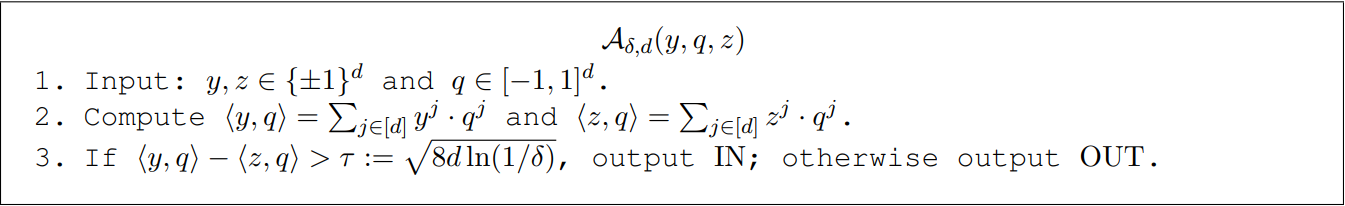
\includegraphics[width=1\textwidth]{im1.png}
		\caption{Hypothesis test of the membership inference attack}
		\label{fig:fig1}
	\end{figure}
	
	I set $d = 2000$, $\delta = 0.05$.Based on \ref{fig:fig1}, the critical value should be 218.93. 
	\begin{lstlisting}[language=Python]	
		significance_level = 0.05
		dimension = 2000
		critical_value = np.sqrt(8 * dimension * np.log(1 / significance_level))		
	\end{lstlisting}	
	  I used the PUMS as the population. Because the algorithm needs the boolean data, we should hash the data. For this purpose, I used boolean projection function from \cite{OpenDPMIA}.
	
	\begin{lstlisting}[language=Python]	
		import numpy as np
		import pandas as pd
		
		def make_boolean_projection(d_in, d_out=1):
			"""Returns a (pseudo)random vector predicate function by hashing data."""
			prime = 691
			desc = np.random.randint(prime, size=(d_in, d_out))
			"""this predicate maps data into a ndarray of booleans of size [n, d_out]	       (where `@` is the dot product and `%` modulus)"""
			return lambda data: ((data.values @ desc) % prime % 2).astype(bool)
		
		population: pd.DataFrame = pd.read_csv(
		"https://raw.githubusercontent.com/opendp/cs208/main/spring2022/data/FultonPUMS5sample100.csv")
		
		projection = make_boolean_projection(len(population.columns), d_out=dimension)
	\end{lstlisting}	
	In each simulation, I took 5 samples as the dataset, and the reference sample should be taken randomly from the population. Under the null hypothesis, the target sample should be taken from the dataset. The utility function simulates output test statistics for a random target sample from the dataset or outside of the dataset and a random reference sample from the population.
	
	\begin{lstlisting}[language=Python]	
		import numpy as np
		import pandas as pd
		
		import numpy as np
		import pandas as pd
		
		def random_dataset(data, sample_size):
		
			"""Returns `sample_size` rows randomly from `data`, and the rest"""
			indices = np.arange(len(data))
			np.random.shuffle(indices)
			
			sampled_data = data.iloc[indices[:sample_size]]
			remaining_data = data.iloc[indices[sample_size:]]
			
			return sampled_data, remaining_data

		 def simulating_function(population,hypothesis="null",sample_size=5):	 
		 
			 dataset, rest_population = random_dataset(population, sample_size)
			 
			 
			 projected_query = projection(dataset).mean(axis=0)
			 
			 
			 projected_reference_sample = projection(population.sample(1).iloc[0])
			 
			 def get_statistics(projected_target_sample, projected_query, projected_reference_sample):
			 
				 projected_target_sample = projected_target_sample * 2 - 1
				 projected_query = projected_query * 2 - 1
				 projected_reference_sample = projected_reference_sample * 2 - 1
				 
				 
				 target_similarity = projected_target_sample.dot(projected_query)
				 reference_similarity = projected_reference_sample.dot(projected_query)
				 statistics = target_similarity - reference_similarity
				 return statistics
			 
			 if hypothesis=="null":
				 projected_target_sample = projection(dataset.sample(1).iloc[0])
				 statistics = get_statistics(projected_target_sample, projected_query, projected_reference_sample)
			 
			 
			 elif hypothesis=="both":
				 statistics = []
				 projected_target_sample = projection(dataset.sample(1).iloc[0])
			 
			 	statistics.append(get_statistics(projected_target_sample, projected_query, projected_reference_sample))
				 projected_target_sample = projection(rest_population.sample(1).iloc[0])
				 statistics.append(get_statistics(projected_target_sample, projected_query, projected_reference_sample))
			 
			 else:
				 projected_target_sample = projection(rest_population.sample(1).iloc[0])
				 statistics = get_statistics(projected_target_sample, projected_query, projected_reference_sample)
			 
			 return statistics
			
	\end{lstlisting} 
	I used "seaborn" package for defining graph function.
	\begin{lstlisting}	
		import seaborn as sns
		
		def graph_function(df):
		plot = sns.histplot(df,kde=True)
		plot.set_xlabel("test statistics")
		plot. axvline(x=critical_value)	
		
	\end{lstlisting} 
		
	 I conduct 1000 simulations under the null hypothesis and plot the histogram of the test statistics.	
	\begin{lstlisting}[language=Python]		
	def simulate(population,hypothesis="null",dimension=100,sample_size=5,num_simulations = 1000):
		all_statistics =[]
		for _ in range(num_simulations):
		all_statistics.append(simulating_function(population,hypothesis,dimension,sample_size))
		return all_statistics
		
		null_list = simulate(population,hypothesis="null",dimension=100,sample_size=5,num_simulations = 1000)
		
		dict = {'null_distribution': null_list} 
		
		df = pd.DataFrame(dict)
		
		graph_function(df)
	
	\end{lstlisting}
	\ref{fig:fig2} shows the null distribution partitioned by the critical region. Statistics greater than the critical value will be correctly accepted, while statistics less than that will lead to the incorrect rejection of the null hypothesis.
	\begin{figure}[h]
		\centering
		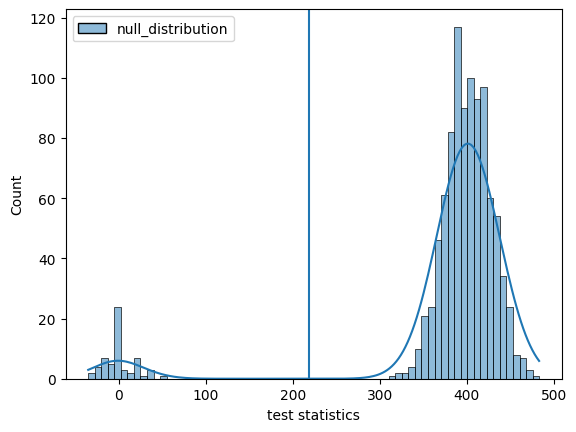
\includegraphics[width=1\textwidth]{im2.png}
		\caption{Null distribution of the test statistics}
		\label{fig:fig2}
	\end{figure}
		\\Now I simulate the complete attack. In one graph two distribution of the test statistics under the null hypothesis and alternative hypothesis is shown.
	
	\begin{lstlisting}[language=Python]	
		   all_list = simulate(population,hypothesis="both",dimension=100,sample_size=5,num_simulations = 1000)
		   
		   dict = {'in_dataset': [l[0] for l in all_list], 'out_dataset': [l[1] for l in all_list]} 
		   
		   df = pd.DataFrame(dict)
		   
		   graph_function(df)
	
	\end{lstlisting}
	\begin{figure}[h]
		\centering
		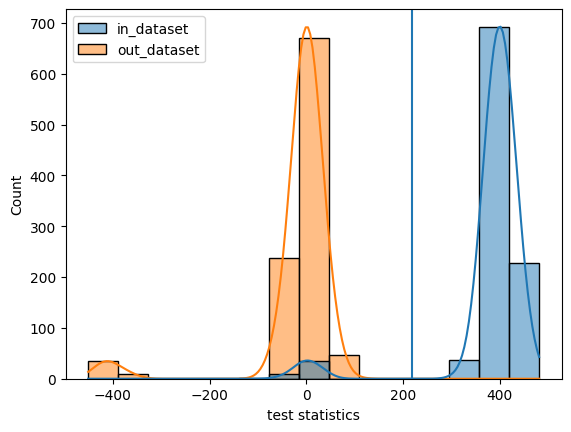
\includegraphics[width=1\textwidth]{im3.png}
		\caption{Null distribution of the test statistics}
		\label{fig:fig3}
	\end{figure}
	\ref{fig:fig3} illustrates the discrimination of test statistics under two hypotheses. The null hypothesis posits that the observation (target sample) is in the dataset, while the alternative hypothesis suggests that the observation does not belong to the dataset. This graph demonstrates the effectiveness of hypothesis testing, as the proportion of samples incorrectly classified as belonging to or not belonging to the dataset is very small.
	\\
	\maketitle{\textbf{Question 2:}}
	First, I built the necessary functions, including a random sampler, calmp, mean query, and Laplace mechanism applied to the mean query.
	\begin{lstlisting}[language=Python]	
		def random_sampler(data,sample_size):
			indices = np.arange(len(data))
			np.random.shuffle(indices)
			sampled_data = data.iloc[indices[:sample_size]]
			return sampled_data
		def clip(dataset,min_margin,max_margin):
			return dataset.clip(min_margin,max_margin)
		def mean_query(dataset):
			return dataset.mean()
		def lap_noise(query,scale):
			return np.random.laplace(query, scale)
		def lap_mech(dataset,epsilon,sensitivity,min_margin=0,max_margin=20):
			scale = sensitivity/epsilon
			cliped_dataset = clip(dataset,min_margin,max_margin)
			query = mean_query(cliped_dataset)
			private_query = lap_noise(query,scale)
			return private_query, query
	\end{lstlisting}
	Next, I downloaded the CSV file and converted it into a Pandas DataFrame. I sampled from the "educ" column of the DataFrame and created a dataset with a size of 500.
	\begin{lstlisting}
		np.random.seed(seed=42)
		sampled_data_frame = random_sampler(data,500)
		sampled_data_set = sampled_data_frame["educ"]
	\end{lstlisting}
	I employed Hamming distance, resulting in a sensitivity of 2 for the histogram. Additionally, I assumed $\epsilon = 0.5$, making the scale of the Laplace noise 4. 
	\begin{lstlisting}[language=Python]	
		# I used hamming distance for neighboring definition, so the sensitivity of the histogram will be 2
		np.random.seed(seed=42)
		epsilon = 0.5
		sensitivity = 2
		scale = sensitivity/epsilon
		max_margin =20
		min_margin = 0
		hist, bins = np.histogram(sampled_data_set, bins =np.arange(min_margin,max_margin)) 
		private_hist = lap_noise(hist,scale).round()
		
		print("Educational level counts:\n", hist)
		print("DP Laplace Educational level counts:\n", private_hist)
		
		df = pd.DataFrame({'bins': bins[:-1], 'hist': hist, 'private hist': private_hist})
		df.plot(x="bins", y=["hist", "private hist"], kind="bar", rot=0)
	\end{lstlisting}
	The true histogram and the private histogram are depicted in \ref{fig:fig4}.
	\begin{figure}[h]
	\centering
	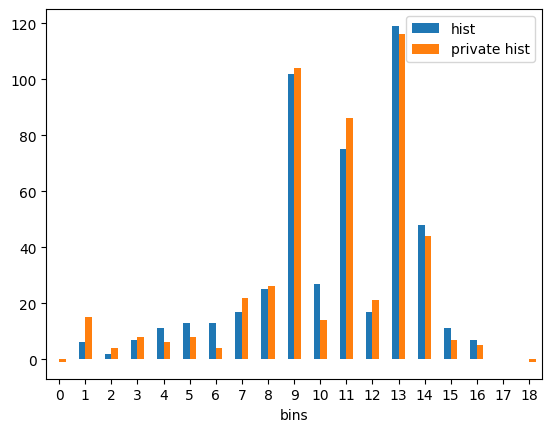
\includegraphics[width=1\textwidth]{im4.png}
	\caption{The true histogram and the private histogram with a Laplace noise scale of 4.}
	\label{fig:fig4}
	\end{figure}\\
	Now I want to use the bootstrap method to sample from the empirical probability mass function of the dataset to create new datasets. First, I grasped the empirical probability mass function.
	\begin{lstlisting}[language=Python]	
		val, cnt = np.unique(sampled_data_set, return_counts=True)
		pmf = cnt / len(sampled_data_set)
		df = pd.DataFrame({'values': val, 'probability': pmf})
		plot = df.plot(x="values", y=["probability"], kind="bar", rot=0)
		plot.set_xlabel("Emprical PMF of the dataset")
	\end{lstlisting}
	 \ref{fig:fig5} shows the empirical probability mass function.
	 \begin{figure}[h]
	 	\centering
	 	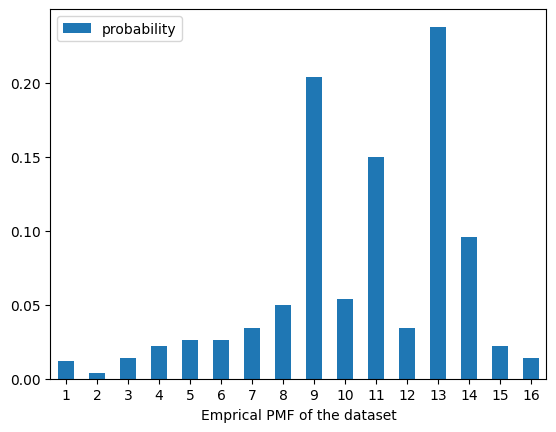
\includegraphics[width=1\textwidth]{im5.png}
	 	\caption{Empirical PMF of the dataset}
	 	\label{fig:fig5}
	 \end{figure}\\
	With the assistance of this distribution, I defined a function for bootstrapping and the Laplace mechanism.
	\begin{lstlisting}[language=Python]
		np.random.seed(seed=42)
		def boot_strap_laplace(val,pmf,epsilon,dataset_size,simulation_number,min_margin=0,max_margin=20) :
			sensitivity = (max_margin - min_margin)/dataset_size
			private_means = []
			true_means = []
			for _ in range(simulation_number):
			rand_data = np.random.choice(val, dataset_size, p=pmf)
			private_mean, true_mean = lap_mech(rand_data,epsilon,sensitivity,min_margin,max_margin)
			private_means.append(private_mean)
			true_means.append(true_mean)
			return sum(private_means)/simulation_number,sum(true_means)/simulation_number
	\end{lstlisting}
	\ref{fig:fig6} plots the error of the Laplace mechanism for the mean query with $\epsilon$ \texttt{= [0.01, 0.05, 0.1, 0.2, 0.3, 0.4, 0.5, 0.6, 0.7, 0.8, 0.9, 1.0]} and dataset sizes $=[5, 10, 20, 50, 100, 200, 500, 1000]$, with a simulation number of 1000 for each $\epsilon$ and dataset size.

	\begin{lstlisting}[language=Python]
		np.random.seed(seed=42)
		epsilons = [0.01,0.05,0.1,0.2,0.3,0.4,0.5,0.6,0.7,0.8,0.9,1.]
		dataset_sizes = [5,10,20,50,100,200,500,1000]
		df = pd.DataFrame(index=epsilons)
		for dataset_size in dataset_sizes:
			all_private_mean = []
			for epsilon in epsilons:
				all_private_mean.append(boot_strap_laplace(val,pmf,epsilon,dataset_size,simulation_number=1000))
			error = [abs(mean[0] - mean[1]) for mean in all_private_mean]
			df[f'Dataset Size={dataset_size}'] = error
		
		plot = df.plot()
		plot.set_xlabel("Epsilon")
		plot.set_ylabel("Absolute Error")
	\end{lstlisting}
	\begin{figure}[h]
		\centering
		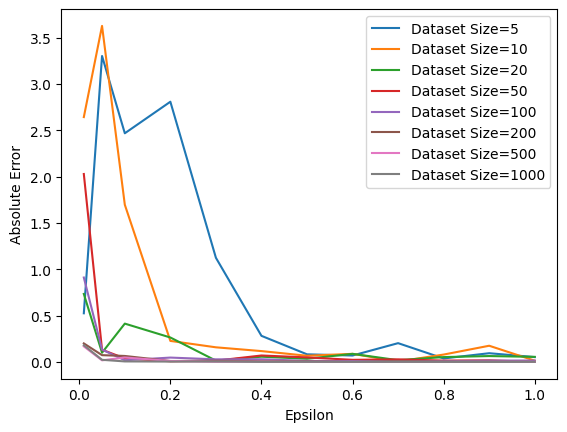
\includegraphics[width=1\textwidth]{im6.png}
		\caption{Absolute error for the range of epsilons and dataset sizes}
		\label{fig:fig6}
	\end{figure}
	\maketitle{\textbf{Question 3:}}
	First I imported packages I need.
	\begin{lstlisting}[language=Python]
		import opendp
		from  opendp import prelude as dp
		from opendp.mod import enable_features
		enable_features('contrib')
	\end{lstlisting}
	
	Then, I downloaded the CSV file and converted the column "educ" to a list. I took this step because when using \texttt{"dp.t.make\_split\_dataframe(separator=",", col\_names=col\_names) >> dp.t.make\_select\_column(key="educ", TOA=str)"}, it was selecting the wrong column, not the "educ" column.
	
	\begin{lstlisting}[language=Python]
		data_list = data["educ"].tolist()
	\end{lstlisting}
	 utilized the input space with the input domain \texttt{"dp.atom\_domain(T=int)" and input metric "dp.symmetric\_distance()"}. Subsequently, I applied \verb|"then_cat_default"| to change the type to float, followed by \verb|"then_clamp"| to restrict the data between 0 and 20. Using \verb|"then_resize"| I created a dataset of 500 samples. Finally, I employed \verb|"then_mean"| to generate the \verb|"sized_bounded_mean"| For the creation of \verb|"base_laplace"| I utilized a scale of $0.5$ and set the output domain and output metric of \verb|"sized_bounded_mean"| as the input domain and input metric for \verb|"base_laplace"| respectively.
	\begin{lstlisting}[language=Python]
		min_margin = 0.
		max_margin = 20.
		edu_bounds =( min_margin,max_margin)
		count_release = 500
		
		input_space = dp.vector_domain(dp.atom_domain(T=int)), dp.symmetric_distance()
		preprocess = (input_space >>
		dp.t.then_cast_default(TOA=float) >>
		dp.t.then_clamp(bounds=edu_bounds) >>
		dp.t.then_resize(size=count_release, constant=10.)) 
		
		true_mean = dp.t.then_mean() 
		sized_bounded_mean = preprocess >> true_mean
		
		base_laplace = dp.m.make_laplace(sized_bounded_mean.output_domain, sized_bounded_mean.output_metric, scale=0.5)
	\end{lstlisting}
	So, the differentially private mean of the dataset, comprising 500 data points, can be shown below.
	\begin{lstlisting}[language=Python]
		# chain with the base_laplace measurement
		dp_mean= sized_bounded_mean >> base_laplace
		
		# release a dp mean
		dp_mean(data_list)
	\end{lstlisting}
	Then, I check if the distance of inputs of the \texttt{"base\_laplace"} is 0.15 based on the input metric (sensitivity). The output distance, based on the output metric ($\epsilon$), will be 0.3 or not.
	\begin{lstlisting}[language=Python]
		# Check that when sensitivity is 0.15, the privacy usage is .30
		base_laplace.check(d_in=.15, d_out=.30)
	\end{lstlisting}
	The output is \texttt{True}. Therefore, with this sensitivity, $\epsilon=0.3$ is achieved because the scale is set to $0.5$. If we increase the sensitivity beyond $0.15$, we can no longer achieve $\epsilon=0.3$. For instance, setting sensitivity to $0.20$ results in an epsilon value greater than $0.4$. The following code yields \texttt{False}.
	\begin{lstlisting}[language=Python]
		base_laplace.check(d_in=.2, d_out=.30) 				
	\end{lstlisting}
	If I set \texttt{max\_influence}, it means that each person only affects one data point. By mapping the transformation \texttt{sized\_bounded\_mean}, we obtain the sensitivity of this transformation. The following code checks whether, when \texttt{max\_influence} is set to 1, the sensitivity is equal to or lower than 0.15.
	\begin{lstlisting}[language=Python]
		max_influence = 1
		eps = 0.3
		sensitivity = 0.15
		sized_bounded_mean.check(d_in=max_influence, d_out=sensitivity) 				
	\end{lstlisting}
	The code above returns \texttt{True}. Now, we examine the privacy expenditure of the entire Laplace mechanism when \texttt{max\_influence} is set to one. The following code also outputs \texttt{True}.
	\begin{lstlisting}[language=Python]
		dp_mean.check(d_in=max_influence, d_out=eps) 				
	\end{lstlisting}
	 I wrote the code below to find the true histogram and private histogram of a random dataset with a sample size of 500, using the \texttt{"then\_count\_by\_categories"} and \texttt{"OpenDP"} package.
	 \begin{lstlisting}[language=Python]
	 	# release a histogram with laplace noise
	 	min_margin = 0
	 	max_margin = 20
	 	categories = [str(category) for category in np.arange(min_margin, max_margin)]
	 	input_space = dp.vector_domain(dp.atom_domain(T=int)), dp.symmetric_distance()
	 	histogram = (input_space >> dp.t.then_cast_default(TOA=float) >>
	 	dp.t.then_resize(size=count_release, constant=10.)>> 
	 	dp.t.then_cast_default(TOA=str) >>
	 	dp.t.then_count_by_categories(categories=categories))
	 	noisy_histogram = histogram >> dp.m.then_laplace(scale=0.5)
	 	hist = histogram(data_list)
	 	private_hist = noisy_histogram(data_list)
	 	
	 	print("Educational level counts:\n", hist[:-1])
	 	print("DP Laplace Educational level counts:\n", private_hist[:-1])
	 	
	 	df = pd.DataFrame({'bins': np.arange(min_margin, max_margin), 'hist': hist[:-1], 'private hist': private_hist[:-1]})
	 	
	 	df.plot(x="bins", y=["hist", "private hist"], kind="bar", rot=0)
	 \end{lstlisting}
	 \ref{fig:fig7} plots true and private histogram with Laplace noise scale of $0.5$.
	 
	 \begin{figure}[h]
	 	\centering
	 	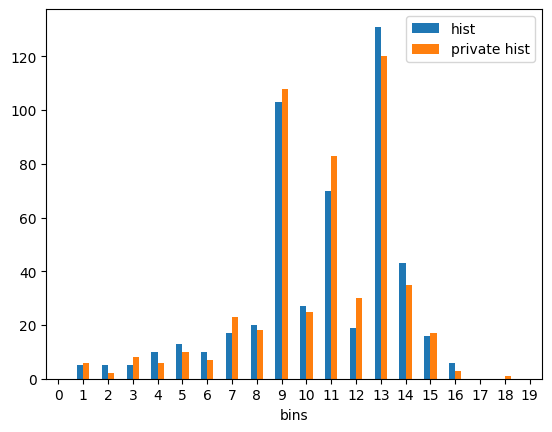
\includegraphics[width=1\textwidth]{im7.png}
	 	\caption{The true histogram and the private histogram generated by \texttt{OpenDP} with a Laplace noise scale of 0.5.}
	 	\label{fig:fig7}
	 \end{figure}
	 Now I do the same for geometric noise of scale 0.5. \ref{fig:fig8} plots true and private histogram with Geometric noise scale of $0.5$.
	 \begin{figure}[h]
	 	\centering
	 	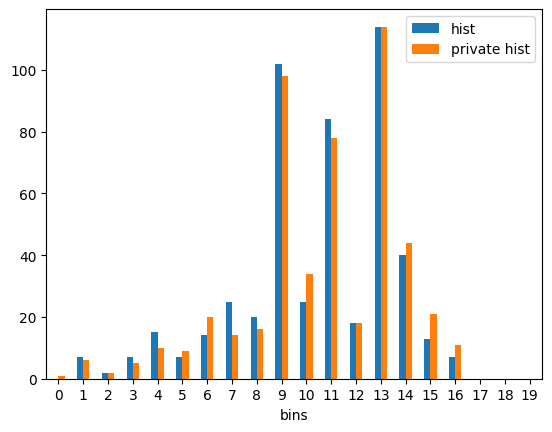
\includegraphics[width=1\textwidth]{im8.png}
	 	\caption{The true histogram and the private histogram generated by \texttt{OpenDP} with a Geometric noise scale of 0.5.}
	 	\label{fig:fig8}
	 \end{figure}
	 \\
	 \maketitle{\textbf{Question 4:}}
	 I followed the same procedure as in \texttt{Question2}, but I constructed the Gaussian mechanism for this question. First, I built the necessary functions, including a random sampler, clamp, mean query, and the Laplace mechanism applied to the mean query.
	 \begin{lstlisting}[language=Python]	
	 	def random_sampler(data,sample_size):
		 	indices = np.arange(len(data))
		 	np.random.shuffle(indices)
		 	sampled_data = data.iloc[indices[:sample_size]]
		 	return sampled_data
	 	def clip(dataset,min_margin,max_margin):
	 		return dataset.clip(min_margin,max_margin)
	 	def mean_query(dataset):
	 		return dataset.mean()
	 	def gaussian_noise(query,variance):
	 		return np.random.normal(query, np.sqrt(variance))
	 	def gaussian_mech(dataset,epsilon,sensitivity,min_margin=0,max_margin=20,delta=1e-8):
		 	variance = (2*np.power(sensitivity,2)*np.log(2/delta))/np.power(epsilon,2)
		 	cliped_dataset = clip(dataset,min_margin,max_margin)
		 	query = mean_query(cliped_dataset)
		 	private_query = gaussian_noise(query,variance)
		 	return private_query, query
	 \end{lstlisting}

	Subsequently, I obtained the CSV file and converted it into a Pandas DataFrame. I then extracted a sample from the "educ" column, resulting in a dataset of 500 entries. Now, I aim to employ the bootstrap method to sample from the empirical probability mass function of the dataset and generate new datasets.
	 \begin{lstlisting}[language=Python]	
		np.random.seed(seed=42)
		sampled_data_frame = random_sampler(data,500)
		sampled_data_set = sampled_data_frame["educ"]
		val, cnt = np.unique(sampled_data_set, return_counts=True)
		pmf = cnt / len(sampled_data_set)
		df = pd.DataFrame({'values': val, 'probability': pmf})
		plot = df.plot(x="values", y=["probability"], kind="bar", rot=0)
		plot.set_xlabel("Emprical PMF of the dataset")
	 \end{lstlisting}[language=Python]
	 \ref{fig:fig9} shows the empirical probability mass function.
	 \begin{figure}[h]
	 	\centering
	 	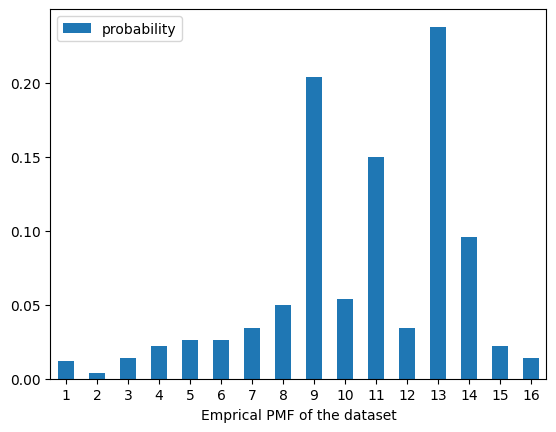
\includegraphics[width=1\textwidth]{im9.png}
	 	\caption{Empirical PMF of the dataset}
	 	\label{fig:fig9}
	 \end{figure}	 
	 Utilizing this distribution, I formulated a function for bootstrapping, incorporating both Laplace and Gaussian mechanisms with a parameter $\delta = 1e-8$.
	 \begin{lstlisting}[language=Python]	
	 	np.random.seed(seed=42)
	 	def boot_strap_gaussian_laplace(val,pmf,epsilon,dataset_size,simulation_number,min_margin=0,max_margin=20) :
		 	sensitivity = (max_margin - min_margin)/dataset_size
		 	private_means_gaussian = []
		 	private_means_laplace = []
		 	true_means = []
		 	for _ in range(simulation_number):
			 	rand_data = np.random.choice(val, dataset_size, p=pmf)
			 	private_mean_gaussian, true_mean = gaussian_mech(rand_data,epsilon,sensitivity,min_margin,max_margin)
			 	private_mean_laplace, _ = lap_mech(rand_data,epsilon,sensitivity,min_margin,max_margin)
			 	private_means_gaussian.append(private_mean_gaussian)
			 	private_means_laplace.append(private_mean_laplace)
			 	true_means.append(true_mean)
		 	return sum(private_means_gaussian)/simulation_number,sum(private_means_laplace)/simulation_number,sum(true_means)/simulation_number
	 \end{lstlisting}
	 In Figure \ref{fig:fig10}, the error of the Laplace mechanism and Gaussian Mechanism for the mean query is plotted with $\epsilon = [0.01, 0.05, 0.1, 0.2, 0.3, 0.4, 0.5, 0.6, 0.7, 0.8, 0.9, 1.0]$ and dataset sizes $=[5, 10, 20, 50, 100, 200, 500, 1000]$. The simulation is conducted 1000 times for each $\epsilon$ and dataset size.
	 \begin{lstlisting}[language=Python]
	 	np.random.seed(seed=42)
	 	epsilons = [0.01,0.05,0.1,0.2,0.3,0.4,0.5,0.6,0.7,0.8,0.9,1.]
	 	dataset_sizes = [5,10,20,50,100,200,500,1000]
	 	df = pd.DataFrame(index=epsilons)
	 	for dataset_size in dataset_sizes:
	 		all_private_mean = []
		 	for epsilon in epsilons:
		 		all_private_mean.append(boot_strap_gaussian_laplace(val,pmf,epsilon,dataset_size,simulation_number=1000))
		 	
		 	error_gaussian = [abs(mean[0] - mean[2]) for mean in all_private_mean]
		 	error_laplace = [abs(mean[1] - mean[2]) for mean in all_private_mean]
		 	df[f'Dataset Size(gaussian,delata=1e-8)={dataset_size}'] = error_gaussian
		 	df[f'Dataset Size(laplace)={dataset_size}'] = error_laplace
	 	
	 	plot = df.plot(figsize=(10, 10))
	 	plot.set_xlabel("Epsilon")
	 	plot.set_ylabel("Absolute Error")
	 \end{lstlisting}
	\begin{figure}[h]
	\centering
	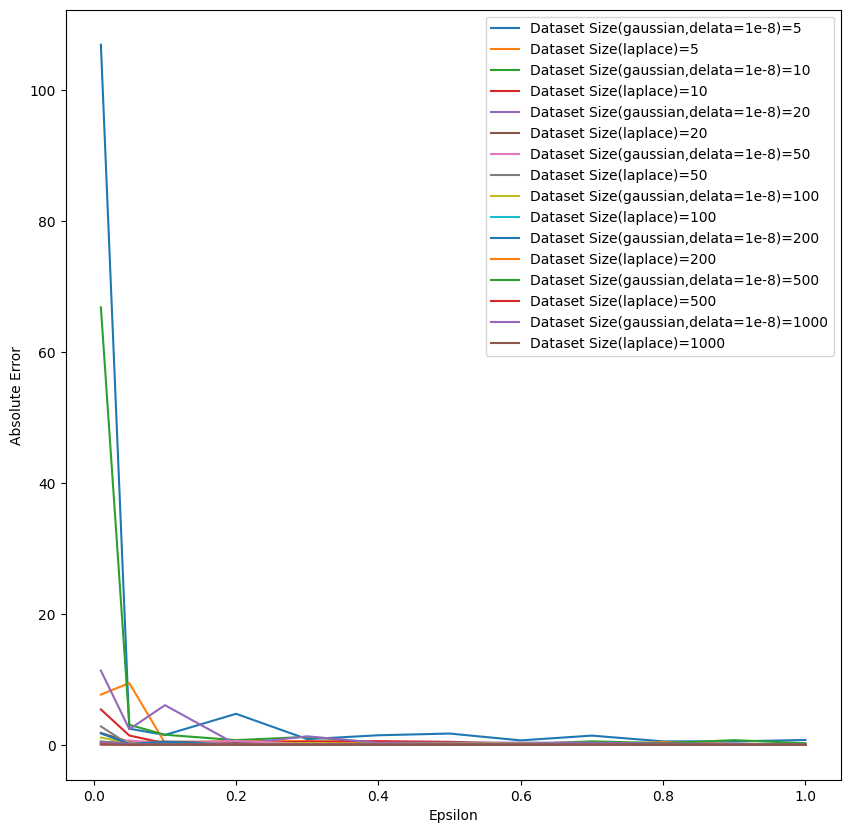
\includegraphics[width=1\textwidth]{im10.png}
	\caption{Absolute error of the Laplace and Gaussian mechanisms for the range of epsilons and dataset sizes}
	\label{fig:fig10}
	\end{figure}
	
	\FloatBarrier
	\bibliographystyle{plain}
	\bibliography{./references}

	
	
	
   \end{document}